\documentclass{article}
\usepackage{float}
\usepackage{graphicx}
\usepackage[margin=1in]{geometry}
\usepackage{amsmath}
\usepackage{relsize}
\newcounter{lecnum}
\usepackage{placeins}

\newcommand{\lecture}[4]{
   \newpage
   \setcounter{lecnum}{#1}
   \noindent

   \begin{center}
   \framebox{
      \vbox{\vspace{2mm}
    \hbox to 16cm { {\bf CS768 Learning with Graphs
                        \hfill 2020-21 Sem I} }
       \vspace{4mm}
       \hbox to 16cm { {\Large \hfill Lecture #1: #2  \hfill} }
       \vspace{2mm}
       \hbox to 16cm { {\it Scribe: #4  \hfill  Lecturer: #3} }
      \vspace{2mm}}
   }
   \end{center}
   \vspace*{4mm}
}

\newtheorem{theorem}{Theorem}[lecnum]
\newtheorem{lemma}[theorem]{Lemma}
\newtheorem{proposition}[theorem]{Proposition}
\newtheorem{claim}[theorem]{Claim}
\newtheorem{corollary}[theorem]{Corollary}
\newtheorem{definition}[theorem]{Definition}
\newtheorem{que}{Que}




\begin{document}

%\lecture{**LECTURE-NUMBER**}{**DATE**}{**LECTURER**}{**SCRIBE**}
\lecture{7}{September 13}{Abir De}{Kaveri Kale}


\section{Supervised Methods For Link Prediction}
In this lecture we saw how to design supervised link predictor. Following are the main tasks in designing supervised link predictor:

\begin{itemize}
  \item Model formulation
  \item Feature construction
  \item Defining loss function
\end{itemize}
\bigskip
%
\paragraph{Designing supervised link predictor:} \\
Consider a social network $G = (V, E)$ in which each edge
$e = (u, v) ∈ E$ represents an interaction between u and
v at a particular time t. Split them into training and testing set.

\begin{eqnarray*}
G_{Training} = (V, T) = (V, E_{Training})
\end{eqnarray*}
 and in Test-set  for each node u we will have 
 $$
\begin{bmatrix} 
Test Edges\\
Test Non-Edges\\
\end{bmatrix}
\quad
$$
In last lecture we already saw Adamic Adar, Preferential Attachment, Common Neighbor which gives the score for edge (u, v), \\
\begin{eqnarray*}
s(u, v) = AA(u, v) \\
s(u, v) = PA(u, v) \\
s(u, v) = CN(u, v)
\end{eqnarray*}
In unsupervised approach, a proximity measure is chosen and used to rank node pairs in the network. The top ranked pairs are predicted to be linked. In the supervised approach, the link prediction is handled as a classification task and different values are used as predictor attributes by a learning algorithm.\\

So we will define new method that is supervised methods where we will combine score from above methods and use them as features for supervised learning. 
\begin{equation} \
\begin{split}
s_W & = W_{AA} AA(u, v) + W_{CN} CN(u, v) + W_{PA} PA(u, v) \\
 & = W^T \begin{bmatrix}
AA(u, v)\\
CN(u, v)\\
PA(u, v)\\
\end{bmatrix}\
\end{split}
\end{equation}
         For each pair (u, v) we can define model,
         \begin{equation} \label{}
\begin{split}
s_w(u, v)  & = W^T \begin{bmatrix}
AA\\
CN\\
PA\\
\end{bmatrix}_{(u, v)}\
\end{split}
\end{equation}
Here $s_W(u, v)$ is parameterized by W and it is stack value of,
   \begin{equation} \label{}
\begin{split}
 W^T =  \begin{bmatrix}
W_{AA}\\
W_{CN}\\
W_{PA}\\
\end{bmatrix}\
\end{split}
\end{equation} 
Don't forget to add bias vector in W.\\
\paragraph{Training the model:} \\
Learn W by training on the available training graph $G_{Training}$. \\
Now, how should we train W?
\paragraph{Example:}
Let consider citation graph which have 2 nodes u and v. And nodes indicates the papers.\\ \\
Define features for each node. \\ \\

u  :- \begin{bmatrix}
f_1 \\
f_2 \\
.\\
.\\
.\\
f_n \\
\end{bmatrix}  \; \& \;
  v :- \begin{bmatrix}
f_1 \\
f_2 \\
.\\
.\\
.\\
f_n \\
\end{bmatrix}

\\ \\
\\where features$ f_1, f_2,...f_n$ could be {tf-idf} of keywords present in paper.\\
\\
Here we can formulate the model,\\
\begin{equation} \
\begin{split}
s_w(u, v) & = Similarity-Index(W .f_u , W.f_v)\\
or \\
s_w(u, v) & = e^{-\alpha{ ||Wf_u - Wf_v||}^2} 
\end{split}
\end{equation}
Here Similarity-Index is some kind of similarity metric, e.g cosine similarity
\begin{equation} \
\begin{split}
cosine-sim(X, Y) & = \frac{X.Y}{||X||_2 ||Y||_2}
\end{split}
\end{equation}
Now define model of scores between u \& v.\\ \\
Given a training graph $ G_{Training} = (V, E_{Training}) $ we can model $s_W(u, v) $ as simple linear predictor.
\begin{equation} \
\begin{split}
s_W(u, v) & = W^T f_{u, v} \\
 & = W^T \begin{bmatrix}
AA(u, v)\\
CN(u, v)\\
PA(u, v)\\
\end{bmatrix}\
\end{split}
\end{equation}
In addition we can define per node features,
\begin{equation} \
\begin{split}
s_W(u, v) & =( W f_u, Wf_v) \\
\end{split}
\end{equation}
For more complicated model simply use complex structure or dependency between two nodes using more "expressive" predictors.\\
\begin{equation} \
\begin{split}
s_\theta(u, v) & =NN_\theta( \{f_u\}, \{f_{u, v}\}) \\
& = FF_\theta( \{f_u\}, \{f_{u, v}\}) \\
\end{split}
\end{equation}
\\
Lets consider $s_W(u, v)$ is linear model and $s_\theta(u, v) $is non-linear model.\\ \\
We have formulated models, now how to train these models? \\
To train we will use supervised approach Support Vector Machine(SVM).\\
\begin{equation} \
\begin{split}
(u, v) \in E \;   s_W(u, v ) \geq 1 - \zeta_{u, v} \\
(u, v) \notin E  \;  s_W(u, v ) \leq 1 - \zeta_{u, v} \\
\end{split}
\end{equation}

Loss function for SVM can be defined as,
\begin{equation} \
\begin{split}
L = \frac{1}{2} \lambda ||W||^2 + (1 - s_W(u, v). Y_{(u, v)})
\end{split}
\end{equation}
where Y is indicator of edge(+1) or non-edge(-1). This loss is called hinge loss. \\ \\
If we combine above two constraint we will get following  form,\\
\begin{equation} \
\begin{split}
Y_{(u, v)}  s_W(u, v ) \geq 1 - \zeta_{u, v} \\
\end{split}
\end{equation}
\begin{figure}[htp]
    \centering
    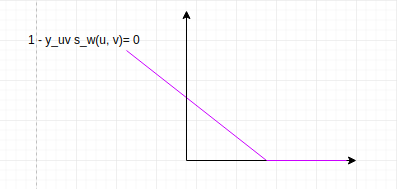
\includegraphics[width=7cm]{hingeloss}
    \caption{Hinge loss}
    \label{fig:hingeloss}
\end{figure}
Here we are trying to construct classifier which will classify edges and non edges.\\
Minimize the loss 
\begin{equation} \
\begin{split}
\sum_{(u,v) \in {Training}}(1 - Y_{(u, v)}  s_W(u, v ))_+  =
&\sum_{(u,v) \in E_{Training}}(1 -  s_W(u, v ))_+  +
\sum_{(u,v) \in  NE_{G}/NE_{Test-set}}(1 +  s_W(u, v ))_+ \\ 
\end{split}
\end{equation}
Once training is done test the model using test-set which contains test-edges and test-non-edges.\\ \\

Caveat : In most graphs
\begin{equation} \
\begin{split}
|E| << |V| \times |V| \\
|E| << |NE|\\
\end{split}
\end{equation}

Data is highly imbalanced. Therefore learning becomes insensitive. \\
In such cases we don't compute loss by above given loss function. Rather we compute $s_W(u, v)$ for edges with $s_W(u, v)$ for non-edges (NE) in  training-set.\\ \\
Consider $(u, v) \in E_{Training} $ and  $  (u^1, v^1) \notin E_{Training},$\\

 \begin{equation} \
\begin{split}
 s_{W}(u, v)  -  s_{W}(u^1, v^1) > 0 \\
 s_{W}(u, v)  >  s_{W}(u^1, v^1)  + \Delta \\
\end{split}
\end{equation}

Loss is greater than 0 iff $ s_{W}(u, v)  <  s_{W}(u^1, v^1)  + \Delta \\$$
\end{document}